% !TeX program = pdflatex
\documentclass[border=6pt]{standalone}
\usepackage{tikz}
\usetikzlibrary{arrows.meta, positioning, calc}

\definecolor{MediumRed}{rgb}{0.925, 0.345, 0.345}
\definecolor{MediumGreen}{rgb}{0.37, 0.7, 0.66}
\definecolor{MediumBlue}{rgb}{0.015, 0.315, 0.45}
\definecolor{DarkBlue}{rgb}{0.05, 0.15, 0.35}

\begin{document}
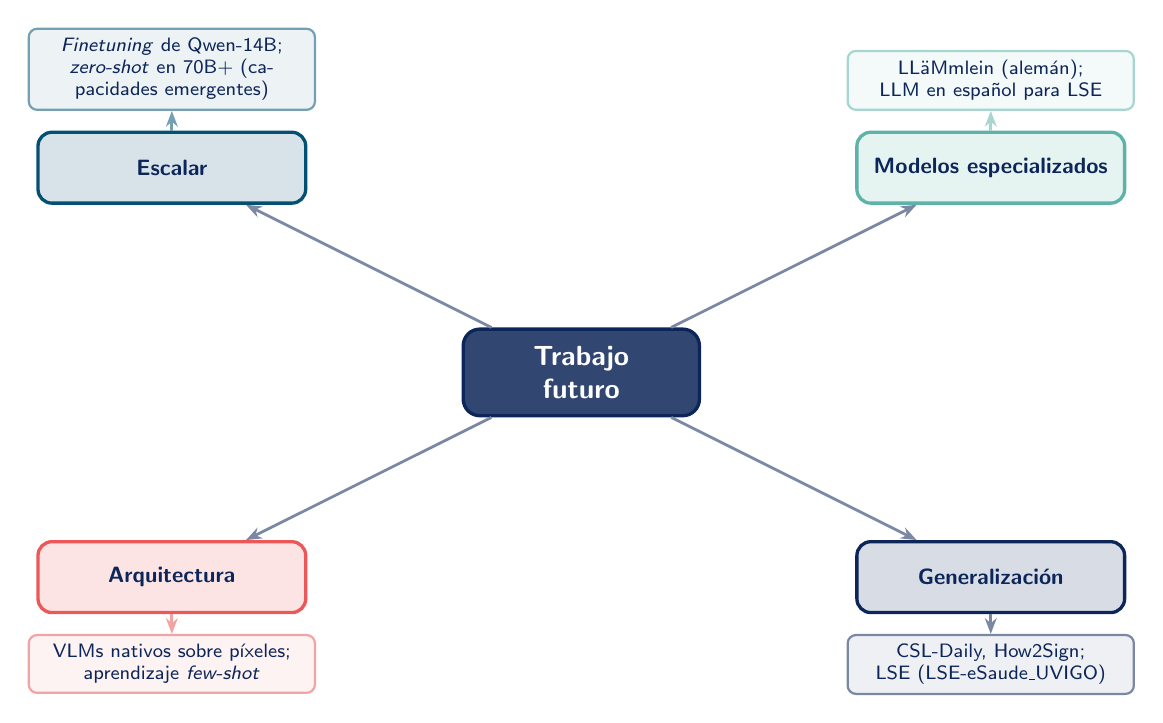
\begin{tikzpicture}[
    font=\sffamily,
    hub/.style={draw=DarkBlue, very thick, rounded corners=6pt, fill=DarkBlue!85, text=white,
        align=center, font=\sffamily\bfseries, minimum width=3.0cm, minimum height=1.1cm},
    theme/.style={draw=#1, very thick, rounded corners=5pt, fill=#1!16, text=DarkBlue,
        align=center, font=\sffamily\footnotesize\bfseries, minimum width=3.4cm, minimum height=0.9cm},
    leaf/.style={draw=#1!55, thick, rounded corners=3pt, fill=#1!7, text=DarkBlue,
        align=center, font=\sffamily\scriptsize, text width=3.4cm},
    link/.style={-{Stealth[length=2mm]}, line width=1pt, DarkBlue!55},
]

% --- nodo central ---
\node[hub] (hub) at (0,0) {Trabajo\\ futuro};

% ================= ESCALA (arriba izq) =================
\node[theme=MediumBlue] (t1) at (-5.2,2.6) {Escalar};
\node[leaf=MediumBlue, above=0.25cm of t1] (l1)
    {\textit{Finetuning} de Qwen-14B; \textit{zero-shot} en 70B+ (capacidades emergentes)};
\draw[link] (hub) -- (t1);
\draw[link, MediumBlue!55] (t1) -- (l1);

% ================= MODELOS ESPECIALIZADOS (arriba der) =================
\node[theme=MediumGreen] (t2) at (5.2,2.6) {Modelos especializados};
\node[leaf=MediumGreen, above=0.25cm of t2] (l2)
    {LL\"aMmlein (alemán); LLM en español para LSE};
\draw[link] (hub) -- (t2);
\draw[link, MediumGreen!55] (t2) -- (l2);

% ================= ARQUITECTURA (abajo izq) =================
\node[theme=MediumRed] (t3) at (-5.2,-2.6) {Arquitectura};
\node[leaf=MediumRed, below=0.25cm of t3] (l3)
    {VLMs nativos sobre píxeles; aprendizaje \textit{few-shot}};
\draw[link] (hub) -- (t3);
\draw[link, MediumRed!55] (t3) -- (l3);

% ================= GENERALIZACION (abajo der) =================
\node[theme=DarkBlue] (t4) at (5.2,-2.6) {Generalización};
\node[leaf=DarkBlue, below=0.25cm of t4] (l4)
    {CSL-Daily, How2Sign; LSE (LSE-eSaude\_UVIGO)};
\draw[link] (hub) -- (t4);
\draw[link, DarkBlue!55] (t4) -- (l4);

\end{tikzpicture}
\end{document}
